\documentclass{article}
\usepackage{fancyhdr}
\usepackage{titlesec}
\usepackage{graphicx}
\usepackage[dvipsnames]{xcolor}
\graphicspath{ {./img/} }
\usepackage{multirow}

\pagestyle{fancy}
\fancyhf{}
\lhead{Modul 5 Praktikum Jaringan Komputer}
\rfoot{\footnotesize Page \thepage}
\lfoot{\footnotesize Mahyus Ihsan, S.Si, M.Si \newline Jurusan Informatika Universitas Syiah Kuala \newline Modul oleh : Diky Wahyudi, Furqan Al Ghifari, Rendika Rahmaturrizki}
\renewcommand{\headrulewidth}{1pt}
\renewcommand{\footrulewidth}{1pt}

\titleformat*{\section}{\small\bfseries}

\begin{document}
    \begin{center}
        \textbf{Modul 5 Praktikum Jaringan Komputer}

        \textbf{IPv6}
    \end{center}

    \section*{Deskripsi Singkat}
    IPv6 adalah versi terbaru dari Protokol Internet, protokol komunikasi yang menyediakan sistem identifikasi dan lokasi untuk komputer di jaringan dan merutekan lalu lintas di Internet. IPv6 dikembangkan oleh Internet Engineering Task Force untuk menangani masalah kelelahan alamat IPv4 yang telah lama diantisipasi. 
    \section*{Tujuan}
    \begin{enumerate}
        \item Dapat memahami struktur dan jenis- jenis dari IPv6
        \item Dapat memahani tentang \textit{subnetting} dan implementasikan pengalamatan pada IPv6
        \item Dapat memahami dan melakukan \textit{Unicast} pada IPv6
    \end{enumerate}

    \begin{flushleft}
        \textbf{Materi 1 - Struktur IPv6}
        \newline

        IPv6 memiliki panjang \textbf{128bits} dan ditulis dalam 8 bagian dan setiap bagian mengandung 16bits yang ditulis dalam 4bit bilangan \textbf{hexadecimal}.

        \begin{center}
            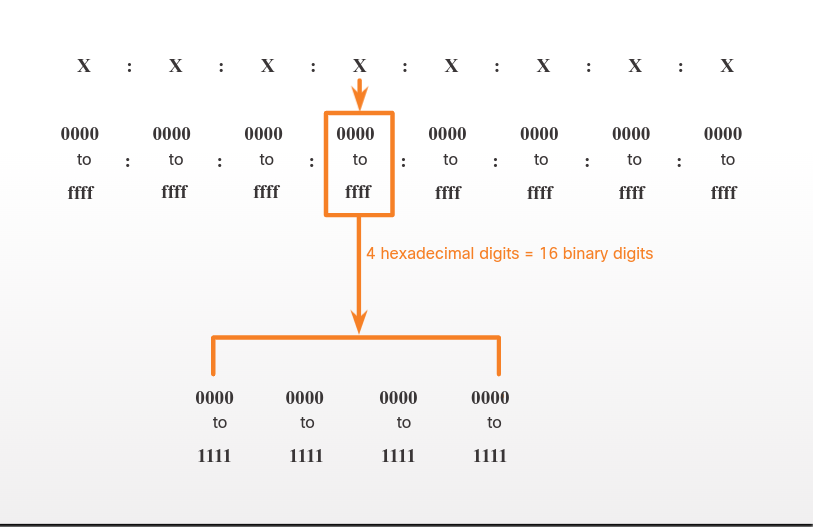
\includegraphics[scale=0.5]{1-1.png}
        \end{center}
        
        Contoh IPv6 
        \begin{center}
            \textbf{2001 : 0db8 : 0000 : 00a3 : ab00 : 0ab0 : 00ab : 1234}
            \newline
        \end{center}

        \textbf{Aturan dalam menulis IPv6}
        \begin{itemize}
            \item[] \textbf{Prefered Format} \newline
            Prefered format adalah cara penulisan IPv6 secara menyeluruh yaitu dengan menggunakan \textbf{32bit bilangan hexadecimal}
            \begin{center}
                2001 : 0db8 : 0000 : 00a3 : ab00 : 0ab0 : 00ab : 1234
            \end{center}
            Semua bit pada IPv6 dituliskan dengan 8 bagian yang antar bagian dibatasi dengan tanda titik koma (;)

            \item[] \textbf{Omit Leading Zeros} \newline
            Omit Leading Zeros adalah pengurangan bilangan 0 yang berada di depan untuk menyingkat penulisan IPv6
            \begin{center}
                2001 : 0db8 : 0000 : 00a3 : ab00 : 0ab0 : 00ab : 1234
            \end{center}
            
            Setelah Omit Leading Zero
            \begin{center}
                2001 : db8 : 0 : a3 : ab00 : ab0 : ab : 1234
            \end{center}

            \item[] \textbf{Double Colon} \newline
            Double Colon adalah penggunaan dua buah tanda titik dua (::) untuk mempersingkat sebuah grup angka 0
            \begin{center}
                2001 : 0db8 : 0000 : 1111 : \textcolor{red}{0000 : 0000 : 0000} : 0200
            \end{center}

            Setelah di sederhanakan menggunakan Omit Leading Zero dan Double Colon akan menjadi
            \begin{center}
                2001 : db8 : 0 : 1111 :: 0200
            \end{center}

            Jika terdapat lebih dari 1 grup angka 0 maka Double Colon akan digunakan pada grup yang paling panjang dan jika mereka sama grup yang pertama kali akan meggunakan Double Colon
            \begin{center}
                2001 : 0db8 : \textcolor{red}{0000 : 0000} : ab00 : \textcolor{red}{0000 : 0000} : 0012
            \end{center}

            Maka akan menjadi
            \begin{center}
                2001 : db8 :: ab00 : 0 : 0 : 12 
            \end{center}
        \end{itemize}
        \newpage
        
        Contoh melakukan \textbf{compress} pada sebuah IPv6
        \begin{itemize}
            \item[] Prefered
            \begin{center}
                2001 : 0db8 : \textcolor{red}{0000 : 0000} : ab00 : \textcolor{red}{0000 : 0000 : 0000}
            \end{center}
            \item[] Omit Leading Zero
            \begin{center}
                2001 : db8 : 0 : 0 : ab00 : 0 : 0 : 0
            \end{center}
            \item[] Double Colon
            \begin{center}
                2001 : db8 : 0 : 0 : ab00 ::
            \end{center}
        \end{itemize}
    \end{flushleft}

    \begin{flushleft}
        \textbf{Materi 2 - Subnetting}
        \newline

        \textbf{Prefix}

        Prefix atau sering juga disebut dengan \textit{network portion} adalah banyaknya host portion yang dapat ditampung oleh sebuah subnet

        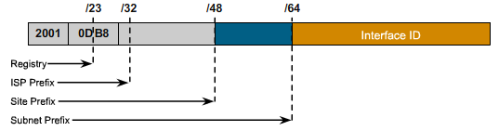
\includegraphics[scale=0.6]{ipv6-structure.png}

        \begin{itemize}
            \item[] \textbf{Registry} \newline
            Adalah IP yang diberikan oleh suatu lembaga kepada pihak yang mengatur jaringan pada suatu wilayah.
            Contoh : APNIC (Asia Pacific Network Information Centre) ke pemerintah Indonesia
            \item[] \textbf{ISP Prefix} \newline
            Adalah IP yang diberikan diberikan oleh lembaga yang mengatur jaringan pada suatu wilayah kepada ISP.
            Contoh : Pemerintah Indonesia ke ISP dari provider seperti Telkom
            \item[] \textbf{Site Prefix} 
            Adalah IP yang diberikan oleh ISP kepada pelanggan dari ISP tersebut.
            Contoh : Telkom ke pelanggan yang menggunakan jaringan melalui pihak telkom.
            \item[] \textbf{Subnet Prefix}
            Adalah IP yang menandakan pembagian dari jaringan yang telah diterima dari ISP.
        \end{itemize}

        Contoh kita akan membuat 3 buah subnet, maka prefix yang digunakan adalah /50 
        Karena kita akan menggunakan 2-bit untuk subnet identifier (48-bit global prefix + 2-bit subnet) dan maximal subnet yang dapat dibentuk dari prefix /50 adalah $2^2 = 4$ subnet

        \begin{center}
            2001:cdba:ac10:\textcolor{red}{0}000:0000:0000:0000:0000
        \end{center}

        untuk bits yang berwarna merah terdapat 4 subnet yaitu

        \begin{itemize}
            \item[] Subnet-0 = \textbf{\textcolor{red}{00}00} = 0
            \item[] Subnet-1 = \textbf{\textcolor{red}{01}00} = 4
            \item[] Subnet-2 = \textbf{\textcolor{red}{10}00} = 8
            \item[] Subnet-3 = \textbf{\textcolor{red}{11}00} = c
        \end{itemize}

        jadi pembagian subnet pada prefix /50 adalah 

        \begin{itemize}
            \item[] Subnet-0 \newline
            Dimulai dari 
            \begin{center}
                2001:cdba:ac10:0000:0000:0000:0000:0000
            \end{center}

            Sampai dengan 
            \begin{center}
                2001:cdba:ac10:3fff:ffff:ffff:ffff:ffff
            \end{center}

            \item[] Subnet-1 \newline
            Dimulai dari 
            \begin{center}
                2001:cdba:ac10:4000:0000:0000:0000:0000
            \end{center}

            Sampai dengan 
            \begin{center}
                2001:cdba:ac10:7fff:ffff:ffff:ffff:ffff
            \end{center}

            \item[] Subnet-2 \newline
            Dimulai dari 
            \begin{center}
                2001:cdba:ac10:8000:0000:0000:0000:0000
            \end{center}

            Sampai dengan 
            \begin{center}
                2001:cdba:ac10:bfff:ffff:ffff:ffff:ffff
            \end{center}
            
            \item[] Subnet-3 \newline
            Dimulai dari 
            \begin{center}
                2001:cdba:ac10:c000:0000:0000:0000:0000
            \end{center}

            Sampai dengan 
            \begin{center}
                2001:cdba:ac10:ffff:ffff:ffff:ffff:ffff
            \end{center}
        \end{itemize}
    \end{flushleft}

    \newpage
    \begin{flushleft}
        \textbf{Materi 3 - Simulasi menggunakan packet tracer}
        \newline

        \begin{enumerate}
            \item Buatlah topologi jaringan seperti pda gambar berikut yang mana terdapat sebuah router, 2 buah switch dan 4 buah pc

            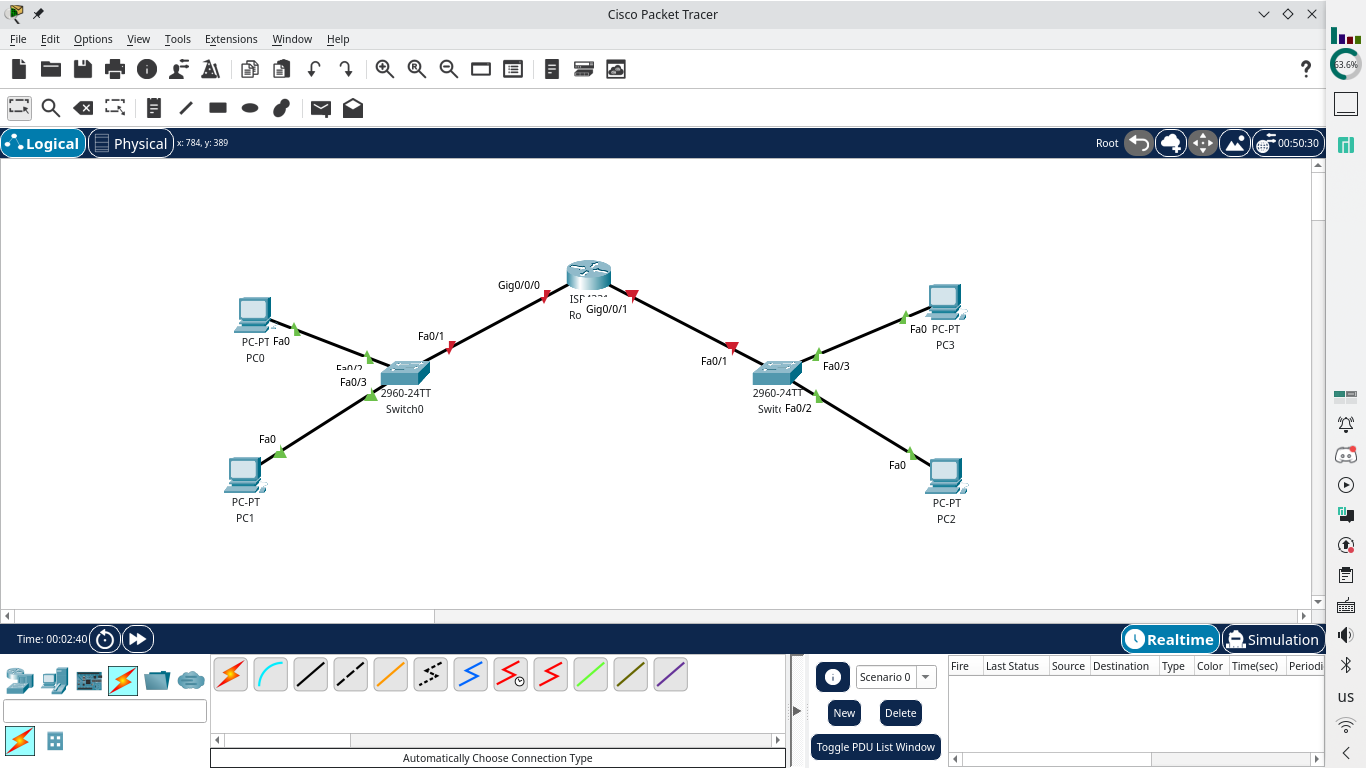
\includegraphics[scale=0.3]{3-1.png}

            \item Berikut tabel ipv6 yang akan digunakan dalam konfigurasi
            \begin{tabular}{|c|c|c|c|}
                \hline
                Device & IPv6 & Interface & Tujuan \\
                \hline
                \multirow{2}{4em}{Router0 }& 2001:cdba:ac10:4000::1/50 & Gigabite0/0/0 & Switch0 \\
                & 2001:cdba:ac10:8000::1/50 & Gigabite0/0/1 & Switch1 \\
                \hline
                PC0 & 2001:cdba:ac10:4000::2/50 & FastEthernet & - \\
                PC1 & 2001:cdba:ac10:4000::3/50 & FastEthernet & - \\
                PC2 & 2001:cdba:ac10:8000::2/50 & FastEthernet & - \\
                PC3 & 2001:cdba:ac10:8000::3/50 & FastEthernet & - \\
                \hline
            \end{tabular}

            \item Pertama kalukan konfigurasi pada PC dengan memberikan ipv6 secara statis, dan lakukanlah dari PC0 hingga PC3 dengan menggunakan ipv6 yang ada pada tabel;

            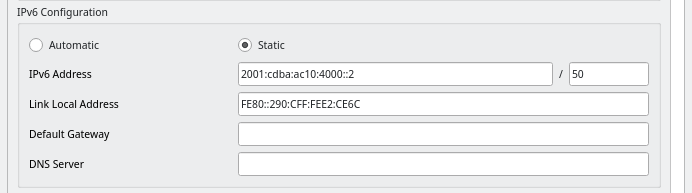
\includegraphics[scale=0.6]{3-2.png}

            \item Setelah memberikan ip pada setiap pc. Uji lah koneksi antar pc yang berada di dalam satu subnet, yaitu PC0 dengan PC1 kemudian PC2 dengan PC3 dengan menggunakan perintah ping
            \newline
            \newline
            
            Ping dari PC0 ke PC1
            \begin{center}
                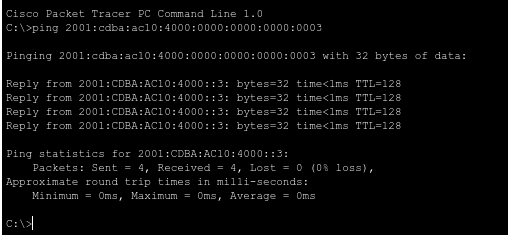
\includegraphics[scale=0.8]{3-3.png}
            \end{center}

            Ping dari PC2 ke PC3
            \begin{center}
                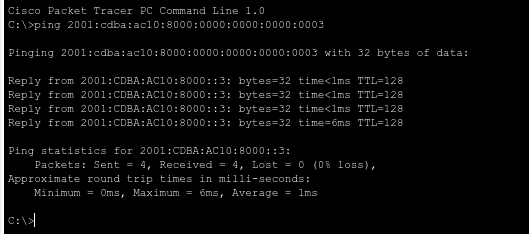
\includegraphics[scale=0.8]{3-4.png}
            \end{center}
                
            \item Jika sudah berhasil, maka setiap perangkat yang berada didalam satu subnet telah terhubung, sekarang koneksikan kedua network dengan menggunakan router.
            
            \item Untuk memberikan IP pada Switch0 menggunakan router bisa dilakukan dengan menggunakan cara berikut
            \item Masuklah ke dalam menu cli pada Router dan masuk ke dalam mode konfigurasi

            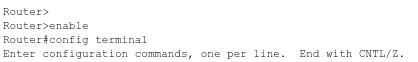
\includegraphics[]{3-5.png}

            \item Kemudian lakukan konfigurasi pada Switch0 yang terhubung melalui port GigabitEthernet0/0/0 dan berikan ip sesuai dengan tabel diatas.
            
            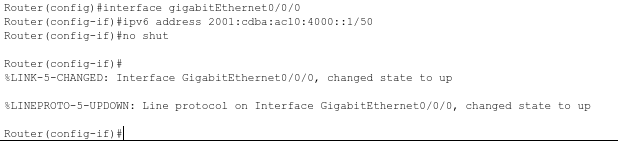
\includegraphics[scale=0.65]{3-6.png}

            \item Dan kemudian dilanjutkan juga dengan Switch1 yang terhubung memalui port GigabitEthernet0/0/1 dan berikan ip sesuai dengan tabel diatas.
            
            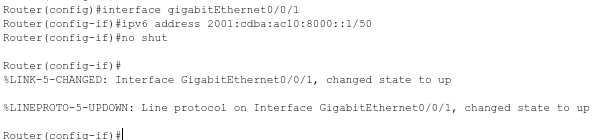
\includegraphics[scale=0.65]{3-7.png}

            \item Setelah selesai memberikan ip pada Switch, jalankan perintah dibawah

            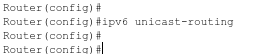
\includegraphics[]{3-8.png}

            \item Setelah kedua network tersambung, maka lakukan konfigurasi gateway pada PC0 hingga PC3. Pada PC0 dan PC1 Switch0 lah yang berperan sebagai Gateway dan pada PC2 dan PC3 Switch1 lah yang berperan menjadi Gateway.
            
            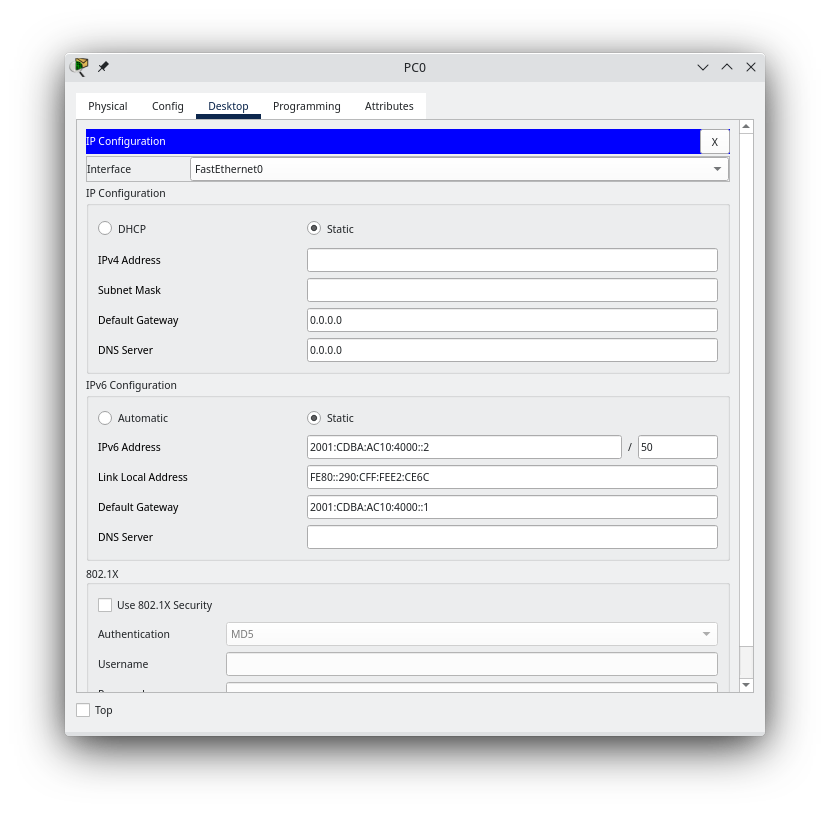
\includegraphics[scale=0.4]{3-9.png}

            \item Setelah melakukan konfigurasi gateway pada semua pc, sekarang lakukan ping dari PC0 atau PC1 ke PC2 atau PC3
            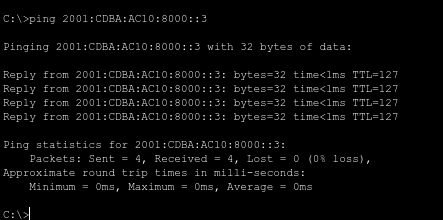
\includegraphics[scale=0.9]{3-10.png}
            Ping dari PC0 ke PC 2, dan PC0 mendapatkan reply dari PC2 maka semua perangkat telah terhubung.
            
        \end{enumerate}
    \end{flushleft}

    \newpage
    \begin{flushleft}
        \textbf{Tugas}
        \newline

        \begin{enumerate}
            \item Sederhanakanlah IPv6 berikut
            \begin{enumerate}
                \item 2001:0000:0db8:1111:0000:0000:0000:0200
                \item 1031:1976:0001:0002:0003:0004:0000:0101
            \end{enumerate}
            \item Tentukanlah banyak subnet dan host yang terbentuk dari
            \begin{enumerate}
                \item 2001:0000:0db8::/51
                \item 2001:0000:0db8::/78
            \end{enumerate}
        \end{enumerate}
    \end{flushleft}
\end{document}
